\documentclass[11pt, UTF8]{ctexart}
% 页面设置
\usepackage{geometry}
\geometry{a4paper, scale=0.8}
\usepackage{fancyhdr}
\pagestyle{plain}
\usepackage{enumitem}
% 符号、字体
\usepackage{amsmath, amssymb, amsthm, bm, mathrsfs}
\usepackage{fontspec}
\newfontface\EmojiFont{Segoe UI Emoji}%[Renderer=HarfBuzz]
\usepackage[dvipsnames]{xcolor}
% 引入图片、绘制矢量图
\usepackage{graphicx}
\graphicspath{ 
  {./images/}
  {../images/} 
}
\usepackage{caption}
\usepackage{subcaption}
\usepackage{tikz, pgf}
\usetikzlibrary{automata, positioning, arrows}
% 代码块
\usepackage{listings}
\usepackage{minted}
\usemintedstyle[cpp]{murphy}
\setminted[cpp]{
  frame = lines,
  framesep = 2mm,
  baselinestretch = 1.2,
  mathescape
}
% 超链接
\usepackage[colorlinks, linkcolor=black]{hyperref}

% 定理环境
\newtheoremstyle{mystyle} % スタイル名
  {}                      % 上部スペース
  {}                      % 下部スペース
  {\normalfont}           % 本文フォント
  {}                      % インデント量
  {\bf}                   % 見出しフォント
  {}                      % 見出し後の句読点, '.'
  { }                     % 見出し後のスペース, ' ' or \newline
  {\underline{\thmname{#1}\thmnumber{#2}\thmnote{(#3)}}}
\theoremstyle{mystyle} % スタイルの適用

\newtheorem{theorem}{定理}[section]
\newtheorem{lemma}{引理}[section]
\renewcommand{\proofname}{证明}

\makeatletter % use at mark
\renewenvironment{proof}[1][\proofname]{\par
  \pushQED{\qed}%
  \normalfont \topsep6\p@\@plus6\p@\relax
  \trivlist
  \item[\hskip\labelsep
        \itshape
    {\bf\underline{#1}}]\ignorespaces
    % {\bf\underline{#1}\@addpunct{.}}]\ignorespaces
}{%
  \popQED\endtrivlist\@endpefalse
}
\makeatother % end at mark

\title{2023集训队选拔赛 个人题解}
\author{Kenshin2438}
\date{2023 年 3 月 13 日}

\begin{document}

\maketitle
\begin{center}
  出于习惯,写个题解(或者叫验题报告)
\end{center}
\tableofcontents
\newpage

\section{干饭协会的入场券{\EmojiFont 🎫}}

使用\texttt{std::STL}容器之前,你应该熟悉它们\textbf{各种操作的复杂度}。\par
将每个$a_i$都分解,相同素数的指数相加得到$n$的分解,最后计算答案。

\section{干饭协会的副本侠{\EmojiFont 😜}}

显然,某一时刻的状态可以通过\textbf{剩余怪兽的数目}和\textbf{当下使用的技能}来确定。由题意可知,该随机过程为马尔可夫过程,即怪兽数目“未来”的状态只取决于“当前”而无关“过去”。\par
用数对\texttt{(number,option)}记录状态,事件A表示使用1技能击杀怪兽,事件B表示使用2技能击杀怪兽,画出其一步转移的状态机如图\ref{fig:StatuGraph}。

\begin{figure}[htbp]
  \centering
  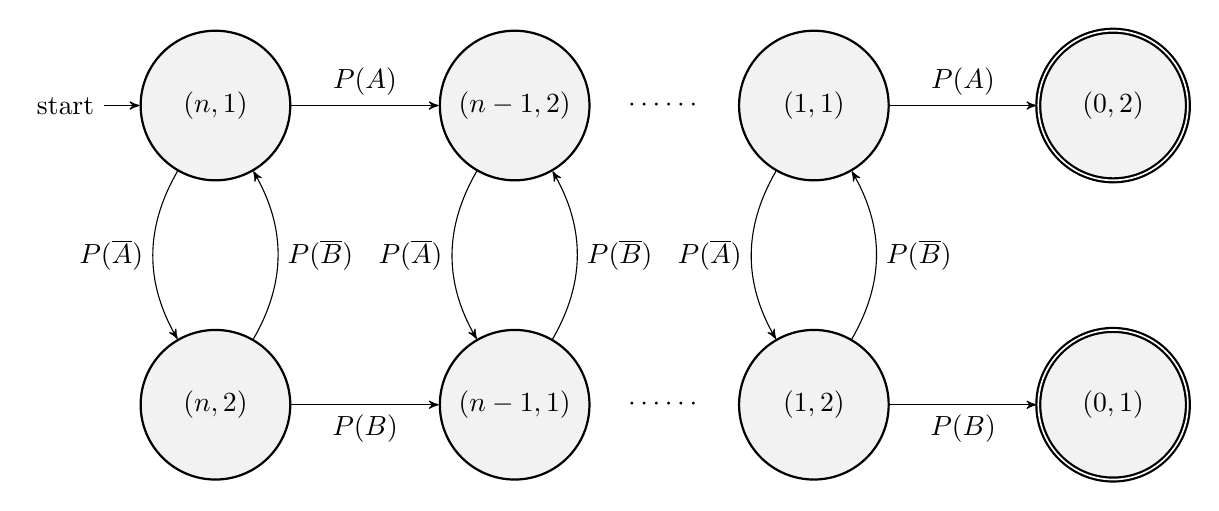
\begin{tikzpicture}[->, >=stealth', node distance=3.8cm]
    \tikzstyle{every state}=[thick, fill=gray!10, minimum size=1.9cm]

    \node[state, initial] (A) {$(n, 1)$};
    \node[state, below of=A] (B) {$(n, 2)$};
    \node[state, right of=A, label=right:$\quad\cdots\cdots$] (C) {$(n - 1, 2)$};
    \node[state, right of=B, label=right:$\quad\cdots\cdots$] (D) {$(n - 1, 1)$};
    \node[state, right of=C] (E) {$(1, 1)$};
    \node[state, right of=D] (F) {$(1, 2)$};
    \node[state, accepting, right of=E] (G) {$(0, 2)$};
    \node[state, accepting, right of=F] (H) {$(0, 1)$};

    \draw (A) edge[bend right, left] node {$P(\overline{A})$} (B);
    \draw (B) edge[bend right, right] node {$P(\overline{B})$} (A);
    \draw (C) edge[bend right, left] node {$P(\overline{A})$} (D);
    \draw (D) edge[bend right, right] node {$P(\overline{B})$} (C);
    \draw (A) edge[above] node {$P(A)$} (C);
    \draw (B) edge[below] node {$P(B)$} (D);

    \draw (E) edge[bend right, left] node {$P(\overline{A})$} (F);
    \draw (F) edge[bend right, right] node {$P(\overline{B})$} (E);
    \draw (E) edge[above] node {$P(A)$} (G);
    \draw (F) edge[below] node {$P(B)$} (H);
  \end{tikzpicture}
  \caption{一步状态转移过程,假定技能1的击杀概率不小于技能2}
  \label{fig:StatuGraph}
\end{figure}

\begin{minted}{cpp}
const function<pair<mint, mint> (int)> E = [&](int n) {
  if (n == 0) return make_pair(mint(0), mint(0));
  const auto &[nE1, nE2] = E(n - 1);
  // $E1 = p1 \times nE2 + (1 - p1) \times E2 + n$
  // $E2 = p2 \times nE1 + (1 - p2) \times E1 + n$
  return make_pair(
    ((p2 * nE1 + n) * (p1 - 1) - (p1 * nE2 + n)) / ((p2 - 1) * (p1 - 1) - 1),
    ((p1 * nE2 + n) * (p2 - 1) - (p2 * nE1 + n)) / ((p1 - 1) * (p2 - 1) - 1)
  );
};
\end{minted}

\section{干饭协会的双子牌{\EmojiFont 🎴}}

DP建议:\textbf{定义清楚状态再写方程}。\par
同\href{https://atcoder.jp/contests/abc291/tasks/abc291_d}{ABC291 D - Flip Cards},官方\href{https://atcoder.jp/contests/abc291/editorial/5861}{题解}。

\section{干饭协会的彩虹猫{\EmojiFont 🐱}}

简单思维。

\section{干饭协会的扮装节{\EmojiFont 🎩}}

最短路。\textbf{Floyd 注意枚举中间点是最外面一层循环}。

\section{干饭协会的招聘书{\EmojiFont 📕}}

典中典的背包问题。注意背包容量大小设置应该不小于$m+\max{f_i}$,或者中间做特殊处理。

\section{干饭协会的捏脸师{\EmojiFont 👩‍🦰}}

\textit{“顾客想把自己的脸型$u$捏成脸型$v$”},意味着捏出$v$就能免费获得$u$。
于是,我们对题目的建图,连接从$v$到$u$的单向边。图中的强连通分量则意味着,只要获得其中任意一个脸谱就能得到该强连通分量的全部脸谱。
强连通分量缩点后,在新图中,没有入度的点意味着必须通过购买获得。\par
\textbf{小细节:}可能出现某张脸谱没有任何人想要,在图中表现为\textbf{单个的点构成的强连通分量}。

\section{干饭协会的排队论{\EmojiFont 📚}}

没有考虑到单调栈这种想法,思维还是受限了。本题的做法应该至少有如下两种:

\subsection*{二分 + 区间最值查询}
本质上就是题意,只是在处理方式上使用了性能优秀的数据结构。如果是线段数维护,还可在线段树上二分(优化$\log$)。

\subsection*{对询问离线}
离线的思想就是,存下所有的询问后,按照最优的顺序而非按照询问的顺序来回答问题。
很难说离线有什么定式,诸君还是要自己把握。\par

还记得我们没考虑的单调栈吗?这种思路很可能源于——只看比当前高度大的就能减少搜索规模(实际并不能)。
不妨我们更进一步——如果队伍中所有点都满足$a[j]>a[pos]+k$就好了。\par

对于询问,$a[pos]+k$是固定的,后面称之为$lim$。
我们只要将$a$数组中大于$lim$的点加入一个\mintinline{cpp}|std::set|,在其中使用\mintinline{cpp}|lower_bound|查询答案。
看似更劣了啊,但是\textbf{不必按询问的顺序}。如果$lim_1>lim_2$,那么满足$a[i]>lim_1$的也一定满足$a[i]>lim_2$。
将询问按$lim$降序排列,则$a$数组中的每一个点都至多加入一次集合。认为$n,q$同级,时间复杂度为$\mathrm{O}(n\log(n))$。

提供一份\href{https://acm.csust.edu.cn/status/49701411403c35a7abe6d619987517ca}{参考代码}

\section{干饭协会的整向量{\EmojiFont ⬅️}}

分类讨论要细致。二元一次方程组,存在无解、多解、唯一解3种情况。\par
\href{https://www.luogu.com.cn/problem/P5656}{P5656 【模板】二元一次不定方程 (exgcd)}

\section{干饭协会的欢乐树{\EmojiFont 🌳}}

DFS序,把子树映射到一段连续区间(时间标号)。注意到,DFS到某点$u$后会将其\textbf{子树}遍历完全。
那么,第一次遇到$u$的时间戳和遍历完子树后重新回到$u$的时间戳之间的时间标号则代表了子树。\par
于是,对于子树的操作变成了区间操作。

\section{干饭协会的签到题{\EmojiFont ✍}}

思维题。

\section{干饭协会的金币树{\EmojiFont 🪙}}

有启发式合并的味道,虽然没有和我一样想法的通过代码。

\section{干饭协会的金手帕{\EmojiFont ✋}}

倍增裸题。

\section{干饭协会的魔法棒{\EmojiFont 🪄}}

线段数维护DP。

\end{document}